\section{Methodology}
\label{sec:method}
% include the figures path relative to the master file
\graphicspath{ {./content/method/figures/} }

% \begin{figure}[t]
%     \centering
%     \begin{subfigure}[b]{0.30\textwidth}
%         \centering
%         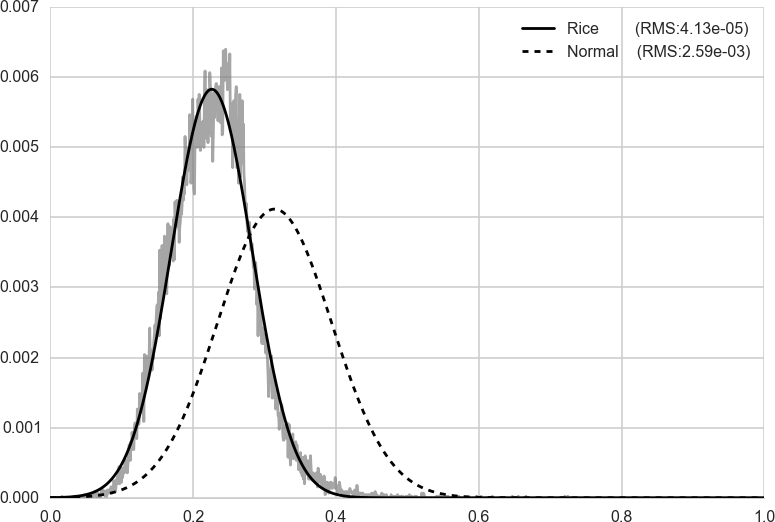
\includegraphics[width=\textwidth]{03}
%     \end{subfigure}
%     \hfill
%     \begin{subfigure}[b]{0.30\textwidth}
%         \centering
%         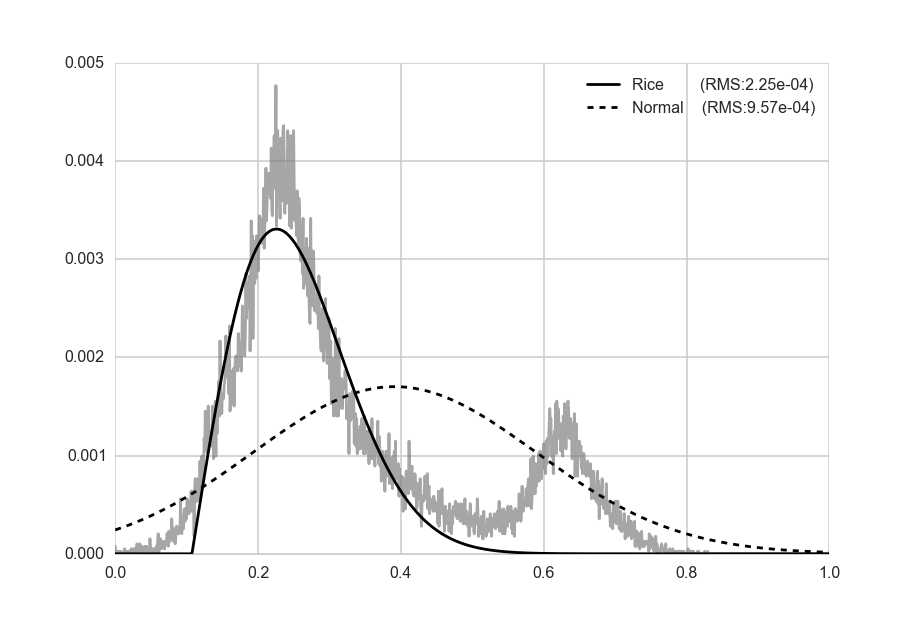
\includegraphics[width=\textwidth]{06}
%     \end{subfigure}
%     \hfill
%     \begin{subfigure}[b]{0.30\textwidth}
%         \centering
%         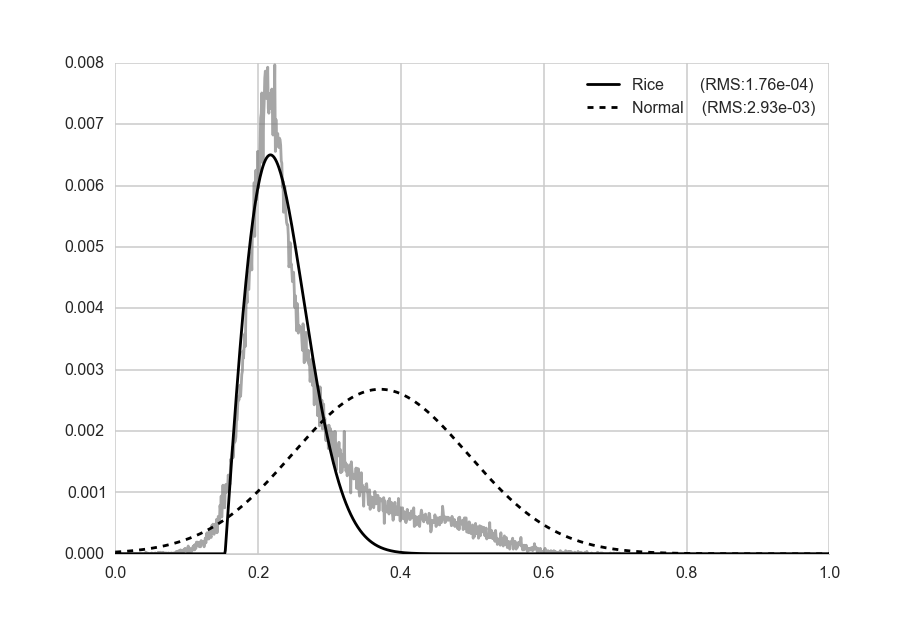
\includegraphics[width=\textwidth]{14}
%     \end{subfigure}
%     \caption {Fitting differences}
%     \label{fig:rice-norm-diff}
% \end{figure}

\begin{figure*}
  \centering
  \subfloat[][]{
    \label{fig:p1}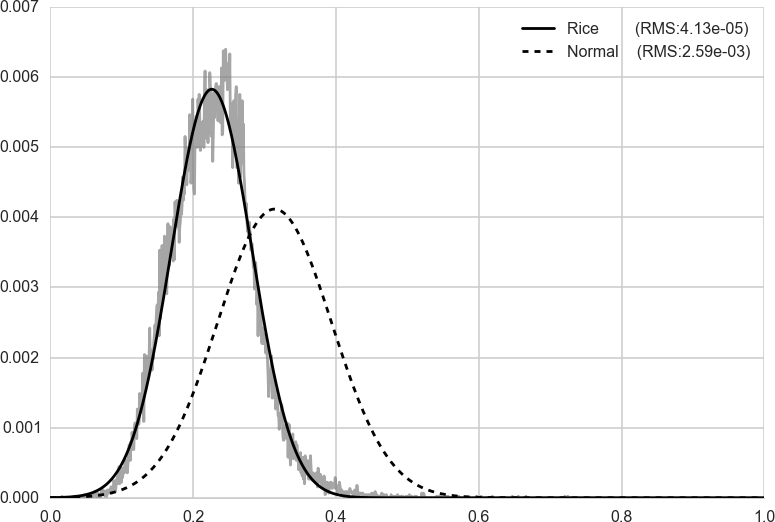
\includegraphics[width=0.3\textwidth]{03}}\hfill
  \subfloat[][]{
    \label{fig:p2}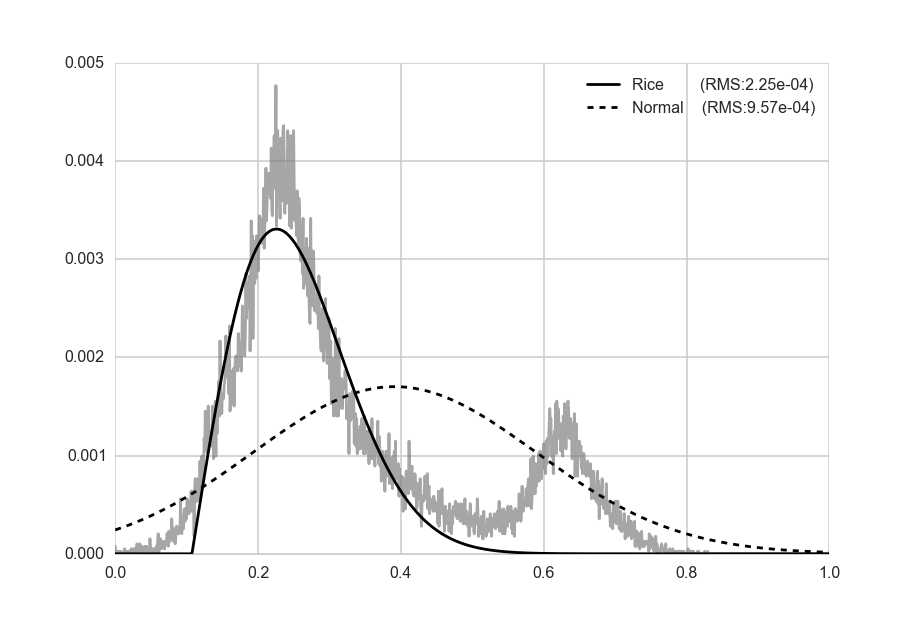
\includegraphics[width=0.3\textwidth]{06}}\hfill
  \subfloat[][]{
    \label{fig:p3}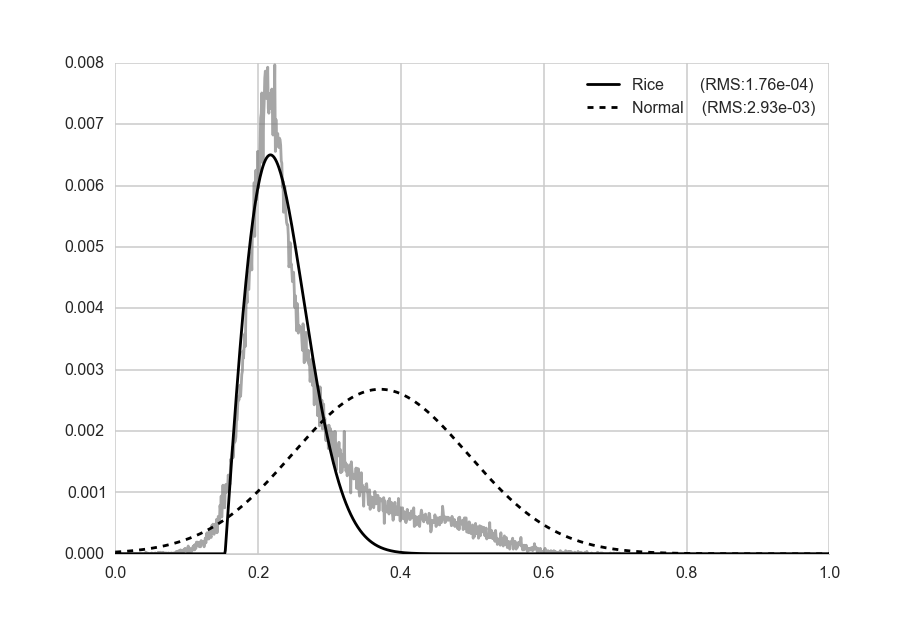
\includegraphics[width=0.3\textwidth]{14}}
  \caption{Visual evaluation of the goodness of fitting using Rician and Gaussian distribution.}
  \label{fig:fitting}
\end{figure*}


%%% Local Variables: 
%%% mode: latex
%%% TeX-master: "../../master"
%%% End: 

